\section{Phase-field approach to fracture}

\subsection{Some words on Griffith's theory of brittle fracture}

In the absence of applied forces, the Griffith theory of brittle
fracture states that \cite{francfort_revisiting_1998}:
(i) The following inequality holds
\begin{equation}
    \begin{aligned}
        G \leq G_{c}
        \mbox{ with }
        G = -\frac{d}{d\Gamma} \int_{\Omega \backslash \Gamma} \frac{1}{2} \tensorii{\varepsilon} : \tensoriv{D} : \tensorii{\varepsilon}
    \end{aligned}
\end{equation}
where $G$ denotes the the elastic energy release rate of the whole structure and $G_c$ is fracture energy.

(ii) That a crack propagation may not occur if the energy release rate is
strictly lower than the fracture energy.

When taking the irreversibility of the crack propagation, the Griffith
theory can be summarised by the following Kuhn-Tucker relations:

\begin{equation}
    \begin{cases}
        \begin{aligned}
            & \dot{\Gamma} \geq 0
            \\
            & G \leq G_{c}
            \\
            & (-G+G_c)\dot{\Gamma} = 0
        \end{aligned}
    \end{cases}
\end{equation}

The Griffith theory have mostly three main flaws \cite{francfort_vers_2002}:
\begin{itemize}
    \item Crack initiation can't be described, as the energy release rate tends
    to zero with the crack surface. Thanks to classical Irwin relations,
    one sees that the energy release rate is related to the stress field
    singularities.
    \item Determination of the crack path requires additional criteria.
    \item Crack propagation must be stable.
\end{itemize}

\subsection{Brittle fracture as an energy minimisation problem}

The variational approach to fracture takes its grounds in the work of
Francfort and Marigo which recasted the Griffith theory into an enery
minimization problem \cite{francfort_revisiting_1998, francfort_vers_2002}:

\begin{equation}
    \label{marigo}
    (\tensori{u} \vert_{t + \Delta t}, \Gamma \vert_{t + \Delta t}) =
    \min_{\tensori{u} \vert_{t}, \Gamma \vert_{t + \Delta t} \supset \Gamma \vert_{t}}
    \int_{\Omega \backslash \Gamma} \frac{1}{2} \tensorii{\varepsilon} : \tensoriv{D} : \tensorii{\varepsilon}
    +
    G_c \Gamma
\end{equation}

% \[
% \paren{\ets{\vec{u}},\ets{\Gamma}}=
% \underset{
% \begin{aligned}
% \vec{u}^{\star}&\in\text{C.A.}\\
% \bts{\Gamma}&\subset\Gamma^{\star}
% \end{aligned}
% }{\argmin{}}
% \int_{\Omega\backslash\Gamma^{\star}}\,\Frac{1}{2}\,\tensorii{\varepsilon}}\supscript{tot}\paren{\vec{u}^{\star}}\,\colon\,\fotensor{D}\,\colon\,\tensorii{\varepsilon}}\supscript{tot}\paren{\vec{u}^{\star}}\,\dtot\,V + G_{c}\,\Gamma^{\star}
% \]{#eq:phase_field:marigo}

Problem \eqref{marigo} is however not tractable with standard
numerical methods \cite{2000_BOURDIN_FRACNFORT_MARIGO_NumericalExperimentsInRevisitedBrittleFracture, chambolle_approximation_2018}, in particular
the commonly used finite element method. For this reason, regularised versions were developed.

% \subsubsection{Regularisation of Problem \eqref{marigo} as a non local damage behaviour}
\subsubsection{Regularisation of the variational problem as a non local damage behaviour}

Following mathematical works of Ambrosio and Tortorelli
\cite{ambrosio1990approximation}, the regularization proposed by Bourdin \textit{et
al.} relies on the following lagrangian \cite{2000_BOURDIN_FRACNFORT_MARIGO_NumericalExperimentsInRevisitedBrittleFracture}:

\begin{equation}
    \label{Bourdin_Lagrangian}
    \begin{aligned}
        \mathcal{L}(\tensori{u},\tensoro{d})
        =
        \int_{\Omega} \rho \psi(\tensorii{\varepsilon}, \tensoro{d})
        +
        \frac{G_c}{c_w} \int_{\Omega}
        \Bigg(
            \frac{w(\tensoro{d})}{\ell}
            +
            \ell \nabla \tensoro{d} \cdot \nabla \tensoro{d}
        \Bigg)
        -
        \mathcal{W}_ext(\tensori{u})
    \end{aligned}
\end{equation}

% \begin{equation}
%     \label{Bourdin_Lagrangian}
%     \mathcal{L}(\vec{u},d) =
%    \int_{\Omega} \rho\psi\paren{\tensorii{\varepsilon}}\supscript{tot},d} \dtot V
%    + \dfrac{G_c}{c_w} \int_{\Omega}\paren{\Frac{w(d)}{l} + l \|\vec{\nabla} d\|^2}\dtot V
%    - \mathcal{W}_{\mathrm{ext}}(\vec{u})
% \end{equation}

where $\tensoro{d} \in [0,1]$ is the damage variable, \textit{i.e.} a continuous field
representing the crack in a \textit{smeared} fashion. The crack position is
lies in the isovalue $\tensoro{d} = 1$, $\rho\psi$ is the part of the free energy coupling elasticity and
damage. $\rho\psi$ is the product a degradation function
$g(d)$ and the free energy $\rho\psi^{\mathrm{el}}$ of an
elastic undamaged material:
\begin{equation}
    \begin{aligned}
        & \rho \psi (\tensorii{\varepsilon}\supscript{tot},d)
        =
        g(\tensoro{d}) \rho \psi^{el}(\tensorii{\varepsilon}\supscript{tot})
        \\
        & \psi^{el}(\tensorii{\varepsilon}\supscript{tot})
        =
        1/2 \tensorii{\varepsilon}\tensorii{\varepsilon}\supscript{tot} : \tensoriv{D} : \tensorii{\varepsilon}\supscript{tot}
    \end{aligned}
\end{equation}

% \begin{equation}
%     \begin{aligned}
%         \rho\psi (\tensorii{\varepsilon}}\supscript{tot},d) = g(\tensoro{d})\,\rho\psi^{\mathrm{el}}\paren{\tensorii{\varepsilon}}\supscript{tot}}\\
%         \rho\psi^{\mathrm{el}}\paren{\tensorii{\varepsilon}}\supscript{tot}}&=\dfrac{1}{2}\,\tensorii{\varepsilon}}\supscript{tot}\,\colon\,\fotensor{D}\,\colon\,\tensorii{\varepsilon}}\supscript{tot}
%     \end{aligned}
% \end{equation}
$g(d)$ is assumed to be a strictly-decreasing function which satisfies
$g(0)=1$ and $g(1)=0$.
$l$ is a small regularization length-scale parameter.
$w(d)$ a strictly-increasing function.
$c_w$ a numerical constant associated with $w$.

As regards the fracture energy density, two choices originating from the
work of Ambrosio and Tortorelli (AT) are widely used, namely:
\begin{itemize}
    \item AT2 model: $w(d) = d^2, c_w=2$.
    \item AT1 model: $w(d) = d, c_w=\dfrac{8}{3}$.
\end{itemize}

The main advantage of the AT1 model is that it exhibits an elastic domain prior damage.

The constant $c_w$ is chosen so that analytical localized solution
profiles correspond to a dissipated energy precisely equal to $G_c$.

The evolution of the displacement $\vec{u}$ and damage field $d$
satisfies the minimisation principle:

\begin{equation}
    \label{phase_field_lagrangian}
    =
    (\tensori{u}\vert_{t + \Delta t}, \tensoro{d}\vert_{t + \Delta t})
    =
    \min_{\hat{\tensori{u}} K.A., \hat{\tensoro{d}} \geq \tensoro{d}\vert_{t}}
    \mathcal{L}(\hat{\tensori{u}}, \hat{\tensoro{d}})
\end{equation}

Problem \eqref{phase_field_lagrangian} typically defines a non local damage
model in the framework of generalised standard materials (see section
). This non local
model can be viewed as a regularisation of a local damage model.

The Lagrangian \eqref{phase_field_lagrangian} uses the first
gradient of damage, but higher order theories may be built as in of the
work of Verhoosel et al. \cite{verhoosel_isogeometric_2011}.

% \subsubsection{About $\Gamma$-convergence}
\subsubsection{About gamma convergence}

Several works have shown, including \cite{2000_BOURDIN_FRACNFORT_MARIGO_NumericalExperimentsInRevisitedBrittleFracture} in the
anti-plane shear case, that the solutions of \eqref{phase_field_lagrangian}
converges in the sense of the so-called $\Gamma$-convergence, to the
solution of the initial Problem \eqref{marigo}.

Those results bridges the conceptual gap between the global approach of
fracture based on Griffith' theory and the local approach to fracture, a
least for a certain class of non local models.

\begin{infobox}{Smeared model}
    The relationship between the smeared model and its parent discrete
    model is corroborated by the proof of the $\Gamma$-convergence result,
    even if it should be emphasized that $\Gamma$-convergence considers
    global minima only, even if fracture mechanics typically deals
    with local minima \cite{freddi_regularized_2010}.
\end{infobox}

\subsubsection{Unilateral effects}
\label{unilateral_effects}

The Lagrangian $\mathcal{L}(u,d)$ can be modified to express the
effect of crack closure, \textit{i.e.} the so-called unilateral effect.

The description of unilateral effects commonly starts by a decomposition
of the elastic energy of an undamaged material into a tensile part
$\rho\psi^{\mathrm{el}}_{+}$ and a compressive part part
$\rho\psi^{\mathrm{el}}_{-}$.

The degradation function is then only applied on the positive part, as
follows:

\begin{equation}
    \rho \psi^{el}(\tensorii{\varepsilon}, \tensoro{d})
    =
    g(\tensoro{d}) \rho \psi^{el}_{+}(\tensorii{\varepsilon})
    +
    \rho \psi^{el}_{-}(tensorii{\varepsilon})
\end{equation}

% % $$
% % \rho\psi^{\mathrm{el}}\paren{\tensorii{\varepsilon}}\supscript{tot},d}=g\paren{d}\,\rho\psi^{\mathrm{el}}_{+}\paren{\tensorii{\varepsilon}}\supscript{tot}}+\rho\psi^{\mathrm{el}}_{-}\paren{\tensorii{\varepsilon}}\supscript{tot}}
% % $$

Here are two classical choices of this decomposition:

\begin{itemize}
    \item A volumetric/deviatoric splitting, as introduced by Amor \textit{et al.}
    \cite{2009_AMOR_MARIGO_MAURINI_RegularizedFormulationOfTheVariationalBrittleFractureWithUnilateralContactNumericalExperiments}:
    \begin{equation}
        \begin{cases}
            \begin{aligned}
                & \rho \psi^{el}_{+}(\tensorii{\varepsilon})
                =
                \frac{1}{2} \kappa \langle \Tr(\tensorii{\varepsilon}) \rangle_{+}^{2}
                +
                \mu \Dev{\tensorii{\varepsilon}} : \Dev{\tensorii{\varepsilon}}
                \\
                & \rho \psi^{el}_{-}(\tensorii{\varepsilon})
                =
                \frac{1}{2} \kappa \langle \Tr(\tensorii{\varepsilon}) \rangle_{-}^{2}
            \end{aligned}
        \end{cases}
    \end{equation}
    with the compression modulus $\kappa = \lambda + 2/3 \mu$.

    % \begin{equation}
    %     \left\{
    %     \begin{aligned}
    %     \rho\psi^{\mathrm{el}}_{+}\paren{\tensorii{\varepsilon}}\supscript{tot}} &= \dfrac{1}{2}\kappa \ppart{\trace{\tensorii{\varepsilon}}\supscript{tot}}}+^2 + \mu
    %     \dev\paren{\tensorii{\varepsilon}}\supscript{tot}}\,\colon\,\dev\paren{\tensorii{\varepsilon}}\supscript{tot}}\\
    %     \rho\psi^{\mathrm{el}}_{-}\paren{\tensorii{\varepsilon}}\supscript{tot}} &=
    %     \dfrac{1}{2}\kappa \npart{\trace{\tensorii{\varepsilon}}\supscript{tot}}}^2
    %     \end{aligned}
    %     \right.
    % \end{equation}
    \item Spectral decomposition, as used by Miehe in the context of the
    variational fracture \cite{2010_MIEHE_HOFACKER_WELSCHINGER_APhaseFieldModelForRateIndependentCrackPropagationRobustAlgorithmicImplementationBasedOnOperatorSplits}:

    \begin{equation}
        \label{spectral_decomposition}
        \begin{cases}
            \begin{aligned}
                & \rho \psi^{el}_{+}(\tensorii{\varepsilon})
                =
                \frac{\lambda}{2} \langle \Tr(\tensorii{\varepsilon}) \rangle_{+}^{2}
                +
                \mu \langle \tensorii{\varepsilon} \rangle_{+} : \langle \tensorii{\varepsilon} \rangle_{+}
                \\
                & \rho \psi^{el}_{-}(\tensorii{\varepsilon})
                =
                \frac{\lambda}{2} \langle \Tr(\tensorii{\varepsilon}) \rangle_{-}^{2}
                +
                \mu \langle \tensorii{\varepsilon} \rangle : \langle_{-} \tensorii{\varepsilon} \rangle_{-}
            \end{aligned}
        \end{cases}
    \end{equation}
    % \begin{equation}
    %     \label{spectral_decomposition}
    %     \left\{
    %     \begin{aligned}
    %     \rho\psi^{\mathrm{el}}_{+}\paren{\tensorii{\varepsilon}}\supscript{tot}} &= \dfrac{\lambda}{2}\, 
    %     \ppart{\trace{\tensorii{\varepsilon}}\supscript{tot}}}^2 + \mu
    %     \ppart{\tensorii{\varepsilon}}\supscript{tot}}\,\colon\,\ppart{\tensorii{\varepsilon}}\supscript{tot}}\\
    %     \rho\psi^{\mathrm{el}}_{-}\paren{\tensorii{\varepsilon}}\supscript{tot}} &= \dfrac{\lambda}{2}\, 
    %     \npart{\trace{\tensorii{\varepsilon}}\supscript{tot}}}^2 + \mu
    %     \npart{\tensorii{\varepsilon}}\supscript{tot}}\,\colon\,\npart{\tensorii{\varepsilon}}\supscript{tot}}\\
    %     \end{aligned}
    %     \right.
    % \end{equation}
\end{itemize}

See also \cite{chambolle_approximation_2018} for some $\Gamma$-convergence
results of these models to an extension of Problem \eqref{marigo}
taking non interpenetration of the crack surfaces.

\subsubsection{Crack nucleation}
\label{crack_nucleation}

Many authors tried to identify the characteristic length $\ell$ as a
material parameter and link it to some observable quantities, such as
the tensile strength $\sigma_{y}$ is the tensile strength.

\begin{equation}
    \begin{aligned}
        \sigma_{y} & =\sqrt{\dfrac{3\,E\,G_{c}}{8\,l}}
        &&
        \text{(AT1)}
        \\
        \sigma_{y} & =\frac{9}{16}\sqrt{\dfrac{E\,G_{c}}{3\,l}}
        &&
        \text{(AT2)}
    \end{aligned}
\end{equation}

This approach has been criticized recently in \cite{kumar_revisiting_2020}.

\subsubsection{Lorentz' variational framework}
\label{lorentz_variational_framework}

Formulation \eqref{phase_field_lagrangian} fits nicely into the variational
framework introduced by Lorentz \textit{et al.}, on the bases established by
Germain et al.
\cite{germain_continuum_1983, lorentz_variational_1999, lorentz_analysis_2003, forest_localization_2004}.
This framework allows properly building various extensions:

\begin{itemize}
    \item unilateral effects, as depicted in Section
    \ref{unilateral_effects}.
    \item cohesive fracture, see \cite{lorentz_convergence_2011, lorentz_nonlocal_2017}.
    \item finite strain modelling.
    \item coupling with other dissipative phenomena (viscoplasticity,
    plasticity, etc.). See for example \cite{2016_ZHANG_These, crabbe_gradient_2018}
\end{itemize}

In particular, the \texttt{ENDO\_SCALAIRE} damage behaviour corresponds to the choice \cite{edf_loi_2011}:

\begin{itemize}
    \item $g(\tensoro{d}) = \Bigg(\frac{1-d}{1+\gamma d}\Bigg)^{2}$ with $\gamma = \frac{3EG_c}{2 \sigma_y \ell} - 1$
    with $\sigma_{y}$ the tensile strength.
    \item $w(\tensoro{d}) = \tensoro{d}$ and $c_w=8/3$, \textit{i.e.} the same choice as for
    the AT1 model.
\end{itemize}

\cite{lorentz_convergence_2011} shows how this behaviour converges to a
cohesive zone model when the characteristic length tends to $0$ in
$1D$, while results in $2D$ may be found in
\cite{cuvilliez_transition_2011}.

\subsection{Numerical strategies}

The reader may refer of Gerasimov and De Lorenzis review which provides
a comprehensive overview of the various numerical approaches available
in the literature \cite{gerasimov_numerical_2020}.

\subsubsection{Weak forms}

Variation of Equation \eqref{phase_field_lagrangian} with respect to the
displacement fields yields the classical principle of virtual work:

\begin{equation}
    \label{pvw}
    \int_{\Omega} \frac{\partial \rho \psi^{el}}{\partial \tensorii{\varepsilon}} : \tensorii{\varepsilon}
    =
    \mathcal{W}_{ext}(\hat{\tensorii{\varepsilon}})
\end{equation}

% \begin{equation}
%     \label{pvw}
%     \int_{\Omega}\deriv{\rho\psi^{\mathrm{e}}}{\tensorii{\varepsilon}}\supscript{tot}}\,\colon\,\tensorii{\varepsilon}}\supscript{tot}\paren{\vec{u}^{\star}}\,\dtot\,V=\mathcal{W}_{\mathrm{ext}}\paren{\vec{u}^{\star}}
% \end{equation}

If we neglect the irreversibility constraint, variation of Equation
\eqref{phase_field_lagrangian} with respect to the damage field yields:

\begin{equation}
    \label{d}
    \int_{\Omega}
    \Bigg(
        \frac{\partial \rho \psi}{\partial d} \hat{\tensoro{d}}
        +
        \frac{G_c}{c_w}
        \Bigg(
            \frac{1}{\ell} \frac{\partial w}{\partial \tensoro{d}} \hat{\tensoro{d}}
            +
            2 \ell \nabla \hat{\tensoro{d}} \cdot \nabla \tensoro{d}
        \Bigg)
    \Bigg)
    = 0
\end{equation}

% \begin{equation}
%     \label{d}
%     \int_\Omega \paren{\deriv{\rho\psi}{d} d^{\star}+\dfrac{G_c}{c_w}\paren{\dfrac{1}{l}\,\derivtot{w}{d}\,d^{\star} + 2\,l \vec{\nabla} d\, \cdot\, \vec{\nabla} d^{\star}}} \,\dtot\,V = 0
% \end{equation}

\begin{infobox}{Analogy with the transient heat equation}
    When the degradation function is quadratic, Equation
    \eqref{d} is formally equivalent to the
    transient heat equation after being discretized
    using a simple backward Euler algorithm.
    This analogy is the basis of the implementations that we developed
    in \texttt{Cast3M}
    \cite{helfer_modelisation_2017, helfer_phase-field_2018, lu_schema_2019}.
\end{infobox}

% > **Analogy with the transient heat equation**
% >
% When the degradation function is quadratic, Equation
% @eq:phase_field:d is formally equivalent to the
% transient heat equation after being discretized
% using a simple backward Euler algorithm.
% This analogy is the basis of the implementations that we developed
% in \texttt{Cast3M}
% \cite{helfer_modelisation_2017, helfer_phase-field_2018, lu_schema_2019}.

\subsubsection{Treatment of the irreversibility constraint}

\paragraph{Constrained minimisation}

Many implementation based on the \texttt{FEniCS} solvers
\cite{alessi_gradient_2015, crabbe_etudes_2017, farrell_linear_2017, bleyer_phase-field_2020}
relies on the \texttt{PETScTAOSolver} optimisation algorithm which allows
finding the solution of the following convex problem:

\begin{equation}
    \tensoro{d}\vert_{d + \Delta t}
    =
    \min_{\hat{\tensoro{d}} \geq \tensoro{d}\vert_{t}}
    \mathcal{L}(\tensori{u}, \hat{\tensoro{d}})
\end{equation}

% \begin{equation}
%     \ets{d} = \underset{d^{\star}\geq\bts{d}}{\argmin{}}\, \mathcal{L}\paren{\vec{u},d^{\star}}
% \end{equation}

where the displacement field $\tensori{u}$ is assumed to be known. This
kind of problem arises naturally when solving Problem
\eqref{phase_field_lagrangian} using a staggered approach, as discussed in
Section XXXX.

\begin{infobox}
    
\end{infobox}

This solver is interfaced by the \texttt{MFrontOptimisationProblem} of the
\texttt{mgis.fenics} python module
\cite{bleyer_overview_2020, bleyer_phase-field_2020} which is part of the
\texttt{MGIS} project \cite{helfer_mfrontgenericinterfacesupport_2020}.

\paragraph{Penalisation}

\cite{gerasimov_penalization_2019}

\paragraph{Lagrange multipliers and active sets}

\cite{heister_primal-dual_2015, jodlbauer_parallel_2020}.

The use of Lagrange multipliers is the basis of the implementation that
we proposed in \cite{helfer_phase-field_2018}. An approximated treatment,
based on the postdoctoral work of Ye Lu, is discussed in Section
XXXX.

\paragraph{Miehe approach \cite{miehe_phase_2010}}

In this section, the specific choice of the free energy is considered:

\begin{equation}
    \rho \psi(\tensorii{\varepsilon}, \tensoro{d})
    =
    (1-\tensoro{d})^2 \rho \psi^{el}_{+}(\tensorii{\varepsilon})
    +
    \rho \psi^{el}_{-}(\tensorii{\varepsilon})
\end{equation}

% \begin{equation}
%     \rho\psi\paren{\tensorii{\varepsilon}}\supscript{tot},d}=\paren{1-d}^{2}\,\rho\psi^{\mathrm{el}}_{+}\paren{\tensorii{\varepsilon}}\supscript{tot}}+\rho\psi^{\mathrm{el}}_{-}\paren{\tensorii{\varepsilon}}\supscript{tot}}\\
% \end{equation}
where $\rho\psi^{\mathrm{el}}_{+}$ and
$\rho\psi^{\mathrm{el}}_{-}$ are given by the Spectral Decomposition
\eqref{spectral_decomposition}.

Departing from the variational framework presented here, Miehe proposed a different treatment of the irreversibility constraint, which consists
in the following modification of Equation \eqref{d}
\cite{miehe_phase_2010}:

\begin{equation}
    \int_{\Omega}
    \Bigg(
        -(1-d)^2 \mathcal{H} \hat{\tensoro{d}}
        +
        \frac{G_c}{c_w}
        \Bigg(
            \frac{1}{\ell}
            \frac{\partial w}{\partial \tensoro{d}} \hat{\tensoro{d}}
            +
            2 \ell \nabla \hat{\tensoro{d}} \cdot \nabla \tensoro{d}
        \Bigg)
    \Bigg)
    = 0
\end{equation}

% \begin{equation}
%     \int_\Omega \paren{-\paren{1-d}\mathcal{H}\widehat{d}+\dfrac{G_c}{c_w}\paren{\dfrac{1}{l}\,\derivtot{w}{d}\,d^{\star} + 2\,l \vec{\nabla} d\, \cdot\, \vec{\nabla} d^{\star}}} \,\dtot\,V = 0
% \end{equation}

where $\mathcal{H}$ is an history field holding the maximum value of
the (undamaged) elastic energy:
\begin{equation}
    \mathcal{H}
    =
    \max_{\tau < t} \rho \psi^{el}_{+}(\tensoro{\varepsilon}(\tau))
\end{equation}
% \begin{equation}
%     \mathcal{H}=\underset{\tau<t}{\max}\, \rho\psi^{\mathrm{el}}_{+}\paren{\tensorii{\varepsilon}}\supscript{tot}\paren{\tau}}
% \end{equation}

Contrary to common beliefs in the litterature, this approach is not
equivalent to Problem \eqref{phase_field_lagrangian}
\cite{gerasimov_numerical_2020}.

However, Miehe' proposal changes the nature of the problem to be solved
from a variational inequality to a variation equality which is:
\begin{itemize}
    \item much more easier to implement or to introduce in standard finite
    element solver.
    \item much more efficient numerically.
\end{itemize}

This explains the success of this proposal which is the basis of most
works made in the phase-field approach of fracture.

\paragraph{Ye Lu' treatment of irreversibility \cite{lu_schema_2019}}
\label{ye_lu_irreversibility}

In an attempt to treat accelerate the treatment of the irreversibility
constraint using Lagrange multipliers, Ye Lu proposed an approximate
treatment of the irreversibility constraint:
\begin{equation}
    \label{ye_lu}
    \tensoro{d}\vert_{t + \Delta t}
    =
    \min_{\hat{\tensoro{d}} > \tensoro{d}_{vert{t}}}
    \mathcal{L}(\tensori{u}, \hat{\tensoro{d}})
\end{equation}
% \begin{equation}
%     \label{ye_lu}
%     \ets{d} = \underset{d^{\star}\geq\bts{d}}{\argmin{}}\, \mathcal{L}\paren{\vec{u},d^{\star}}
% \end{equation}

where the displacement field $\tensori{u}$ is again assumed to be known.

Problem \eqref{ye_lu} is solved iteratively. At each iteration,
a Dirichlet condition, enforcing the constraint
$\tensoro{d}\supscript{i} = \tensoro{d}\vert_{t}$, is
added to each nodes which does not respect the condition
$\tensoro{d}\supscript{i} \geq \tensoro{d}\vert_{t}$. Contrary to the active set algorithm, this
constraint is not removed during the iterations. Iterations are stopped
when every node satisfies the irreversibility constraint.

Ye Lu observed a significant decrease of the computational time when
compared to the use of the active set method, as implemented in
\texttt{Cast3M}.

Moreover, the approximated treatment of the irreversibility constraint
seems to be compensated by the fact that the Problem
\ref{ye_lu} is part of a staggered approach which is described
in Section \ref{castem_implementation}. Although no proof can
be established that the converged solution of this staggered approach
with this approximated treatment of the irreversibility is equivalent of
a rigorous resolution of Problem \ref{phase_field_lagrangian}, numerical
results are encouraging \cite{lu_schema_2019}.

\paragraph{Monolithic resolution}

\begin{figure}[h!]
    \centering
    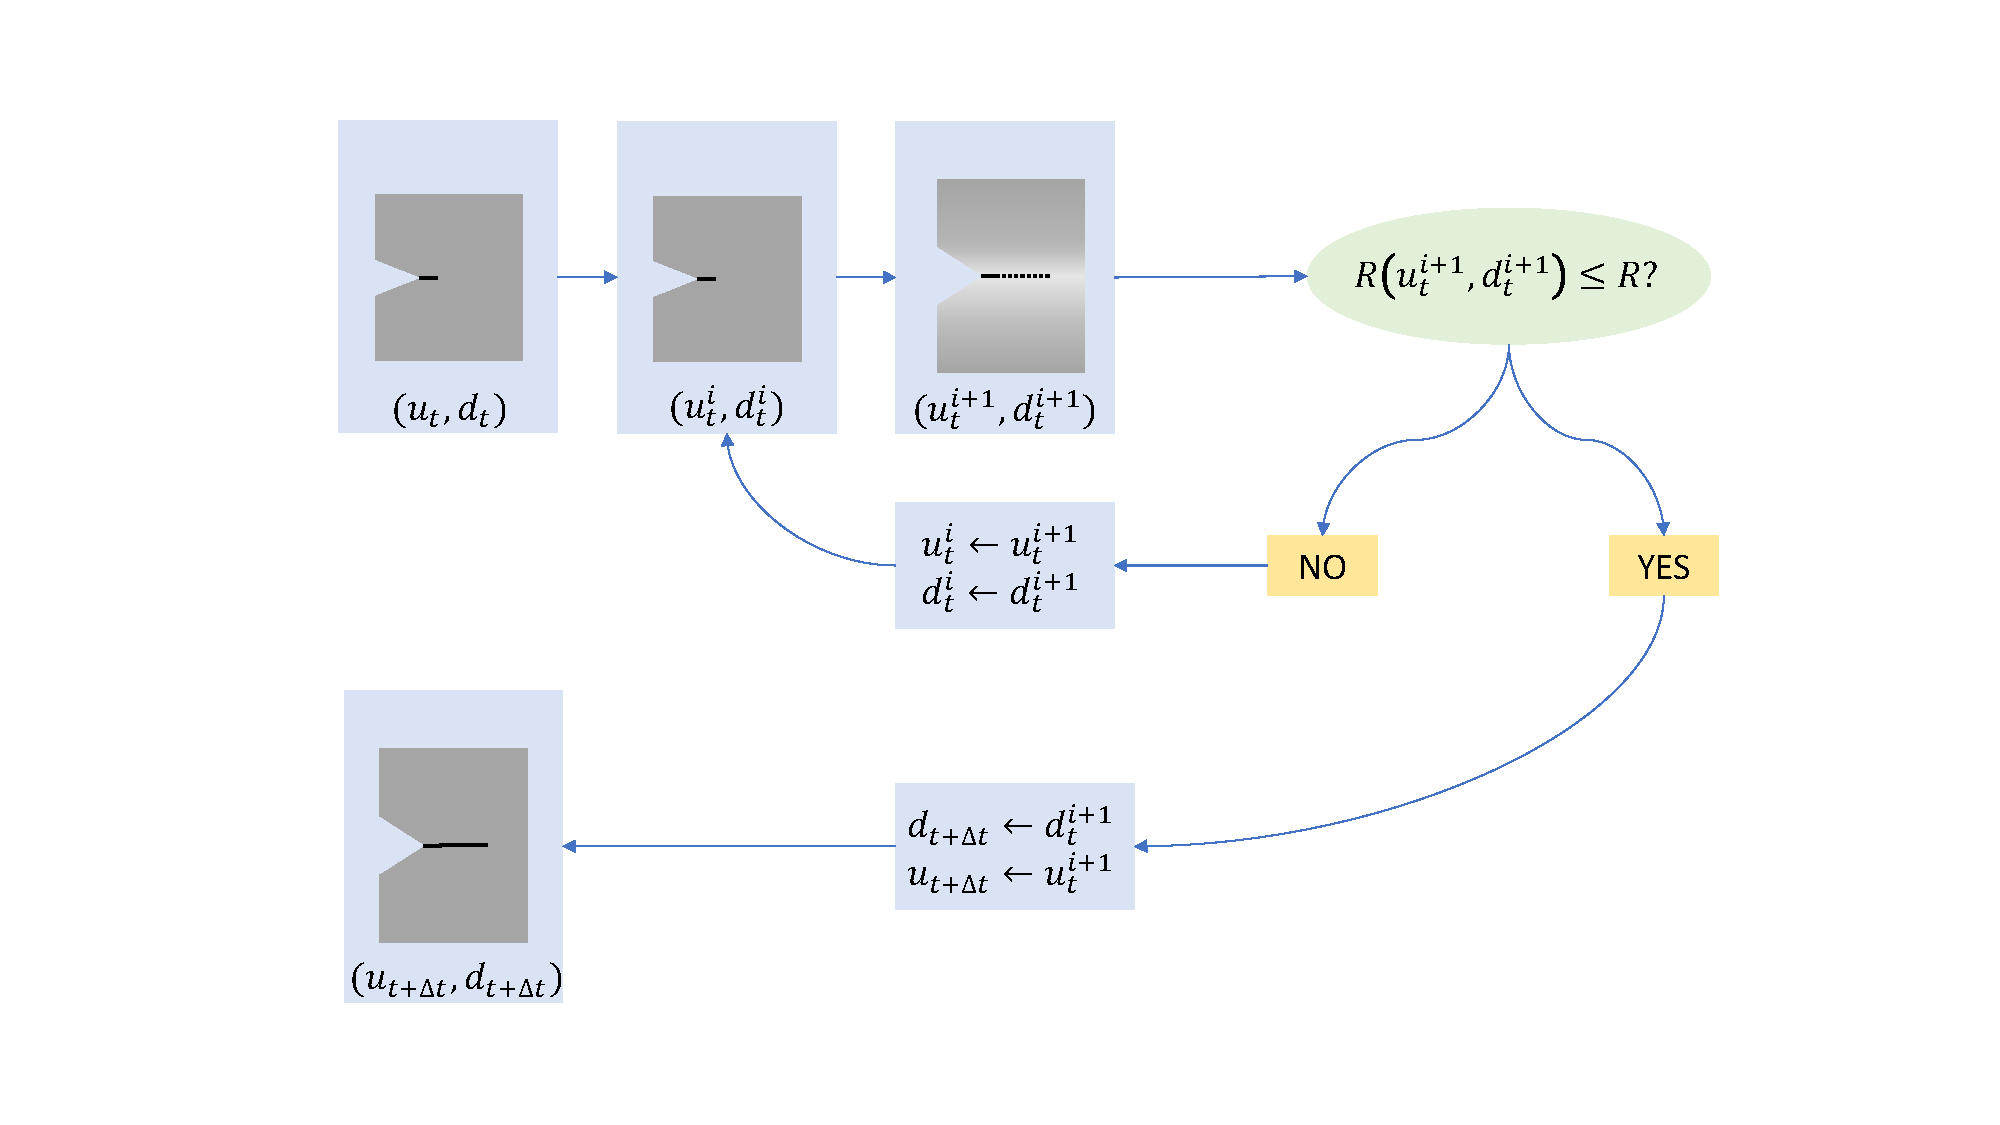
\includegraphics[width=7.cm]{img/monolithic-resolution.pdf}
    \caption{Illustration of the monolithic resolution of Problem \ref{phase_field_lagrangian}}
    \label{phase-field}
\end{figure}

% ![Illustration of the monolithic resolution of Problem @eq:phase_field_lagrangian.](img/phase-field/)

\cite{wick_modified_2017, edf_modelisation_2019}

\subsubsection{Staggered resolution}
\label{staggered_resolution}

Staggered resolutions are based on the idea of solving Problem
\ref{phase_field_lagrangian} alternatively:

\begin{itemize}
    \item for the displacement field (at constant damage field):
    \begin{equation}
        \label{problem_u}
        % \vec{u} = \underset{\vec{u}^{\star}\in\text{C.A.}}{\argmin{}}\, \mathcal{L}\paren{\vec{u}^{\star},d_\mathrm{fixed}}
        \tensori{u}
        =
        \min_{\hat{\tensori{u}} K.A.} \mathcal{L}(\tensori{u}, \tensoro{d}_{fixed})
    \end{equation}
    \item for the damage field (at constant displacement field):
    \begin{equation}
        \label{problem_d}
        \tensoro{d}
        =
        \min_{\hat{\tensoro{d}} \geq \tensoro{d}\vert_{t}} \mathcal{L}(\tensori{u}\subscript{fixed}, \tensoro{d}_{fixed})
        % d = \underset{d^{\star}\geq\bts{d}}{\argmin{}}\, \mathcal{L}\paren{\vec{u}_\mathrm{fixed},d^{\star}}
    \end{equation}
\end{itemize}

Note that Problems \ref{problem_u} and
\ref{problem_d} are convex.

\paragraph{Alternate minimisation}

% ![Illustration of the alternate minimisation algorithm applied to Problem @eq:phase_field_lagrangian.](img/phase-field/alternate-minimisation-resolution.pdf)

\begin{figure}[h!]
    \centering
    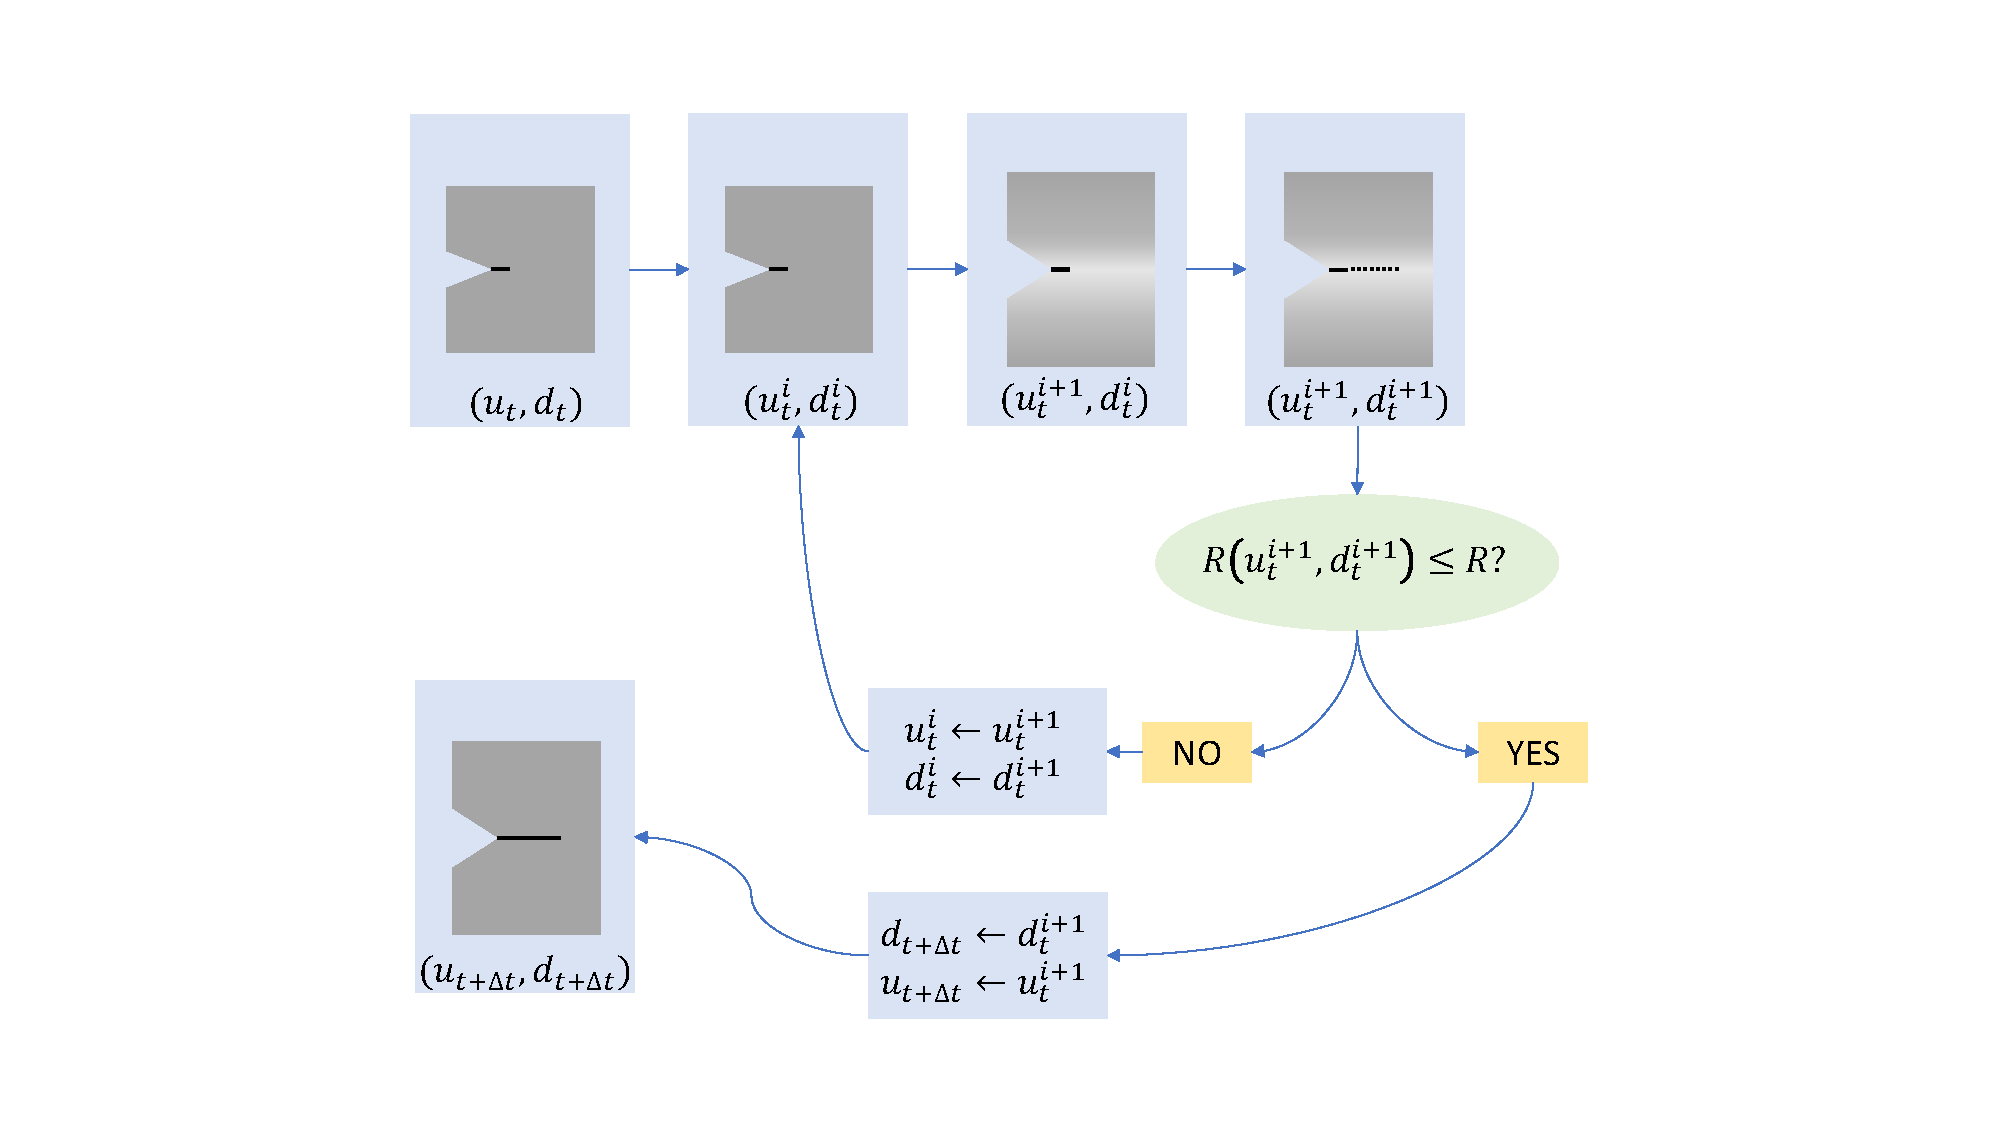
\includegraphics[width=7.cm]{img/alternate-minimisation-resolution.pdf}
    \caption{Illustration of the alternate minimisation algorithm applied to Problem \ref{phase_field_lagrangian}}
    \label{alternate_minimisation_resolution}
\end{figure}

The alternate minimisation algorithm, introduced by Bourdin \textit{et al.}
\cite{2000_BOURDIN_FRACNFORT_MARIGO_NumericalExperimentsInRevisitedBrittleFracture}, uses a fixed point algorithm to find a pair
$\tensori{u}\vert_{t+\Delta t}, \tensoro{d}\vert_{t+\Delta t}$
% $\ets{\vec{u}},\ets{d}$
which satisfies both Problems
\ref{problem_u} and \ref{problem_u}, \textit{i.e.} is a
solution of the initial Problem \ref{phase_field_lagrangian}.

At the $i^{\text{th}}$ iteration, the current estimate of the
displacement field
% $\ets{\vec{u}}^{(i)}$
$\tensori{u}\vert_{t+\Delta t}\supscript{(i)}$
is used to get a new estimate
% $\ets{d}^{(i+1)}$
$\tensoro{d}\vert_{t+\Delta t}\supscript{(i+1)}$
of the damage field which is then used to get a new
estimate
% $\ets{\vec{u}}^{(i+1)}$
$\tensori{u}\vert_{t+\Delta t}\supscript{(i+1)}$
of the displacement field, as
follows:
\begin{equation}
    \begin{cases}
        \begin{aligned}
            \tensoro{d}\vert_{t+\Delta t}\supscript{(i+1)}
            =
            \min_{\hat{\tensoro{d}} \geq \tensoro{d}\vert_{t}}
            \mathcal{L}(\tensori{u}\vert_{t + \Delta t}^{i}, \hat{\tensoro{d}})
            \\
            \tensori{u}\vert_{t+\Delta t}\supscript{(i+1)}
            =
            \min_{\hat{\tensori{u}} K.A.}
            \mathcal{L}(\hat{\tensori{u}}, \tensoro{d}\vert_{t + \Delta t}^{i+1})
        \end{aligned}
    \end{cases}
\end{equation}

% \begin{equation}
%     \left\{
%     \begin{aligned}
%     \ets{d}^{(i+1)}       &= \underset{d^{\star}\geq\bts{d}}{\argmin{}}\, \mathcal{L}\paren{\ets{\vec{u}}^{(i)},d^{\star}}\\
%     \ets{\vec{u}}^{(i+1)} &= \underset{\vec{u}^{\star}\in\text{C.A.}}{\argmin{}}\, \mathcal{L}\paren{\vec{u}^{\star},\ets{d}^{(i+1)}}
%     \end{aligned}
%     \right.
% \end{equation}

As the Lagrangian
% $\mathcal{L}\paren{\ets{\vec{u}}^{(i+1)},\ets{d}^{(i+1)}}$
$\mathcal{L}(\tensori{u}\vert_{t + \Delta t}^{i+1}, \tensoro{d}\vert_{t + \Delta t}^{i+1})$
has a lower value than
% $\mathcal{L}\paren{\ets{\vec{u}}^{(i)},\ets{d}^{(i)}}$
$\mathcal{L}(\tensori{u}\vert_{t + \Delta t}^{i}, \tensoro{d}\vert_{t + \Delta t}^{i})$
,
this algorithm does converge to a solution of Problem
\ref{phase_field_lagrangian}.

However, the number of fixed point iterations is generally very
important. Farrell \textit{et al.} showed how this algorithm may be accelerated
significantly \cite{farrell_linear_2017}.

\paragraph{Time staggered}

% \begin{figure}[h!]
%     \centering
%     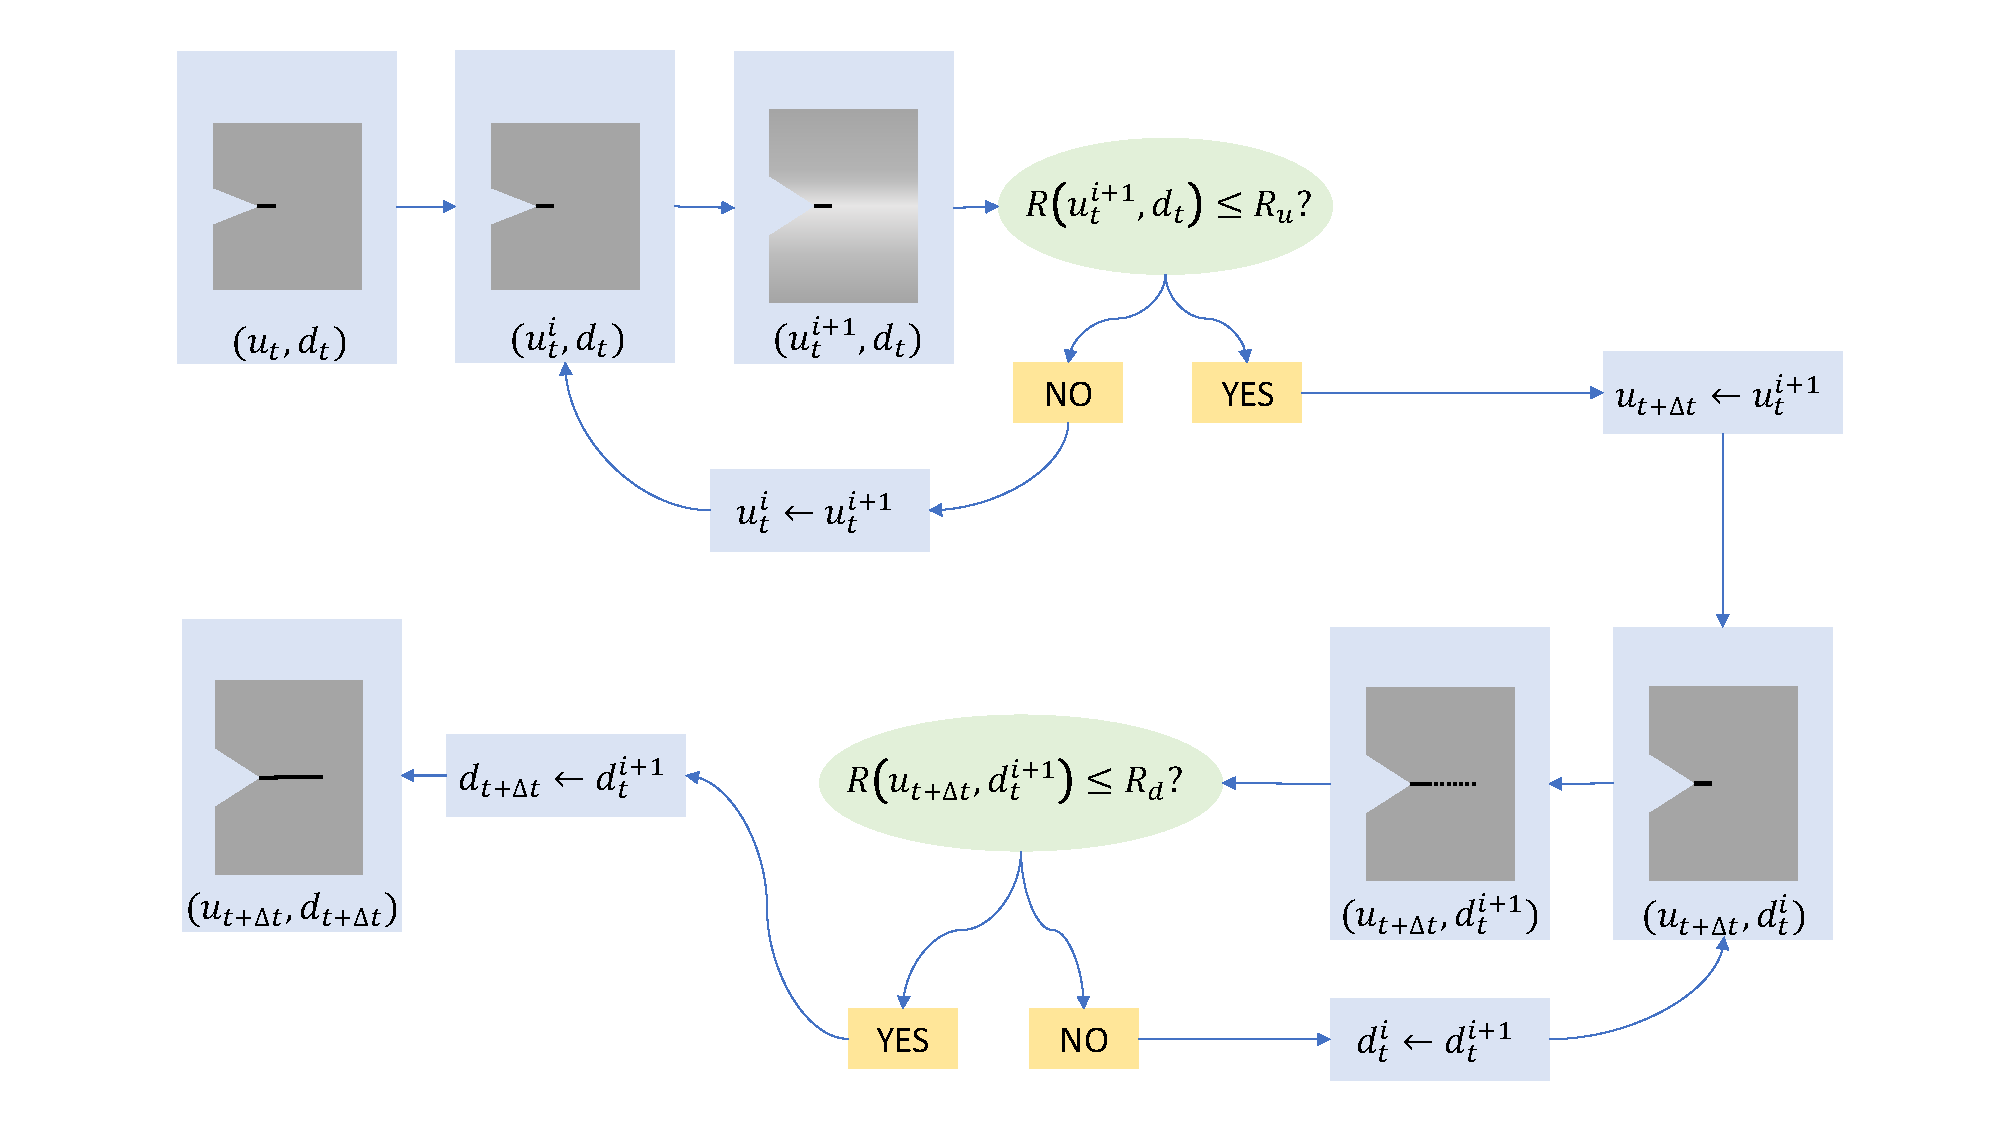
\includegraphics[width=7.cm]{img/time-staggered-resolution.pdf}
%     \caption{Illustration of the time staggered resolution of Problem \ref{phase_field_lagrangian}}
%     \label{time_staggered_resolution}
% \end{figure}

% ![Illustration of the time staggered resolution of Problem @eq:phase_field_lagrangian.](img/phase-field/time-staggered-resolution.pdf)

\begin{figure}[h!]
    \centering
    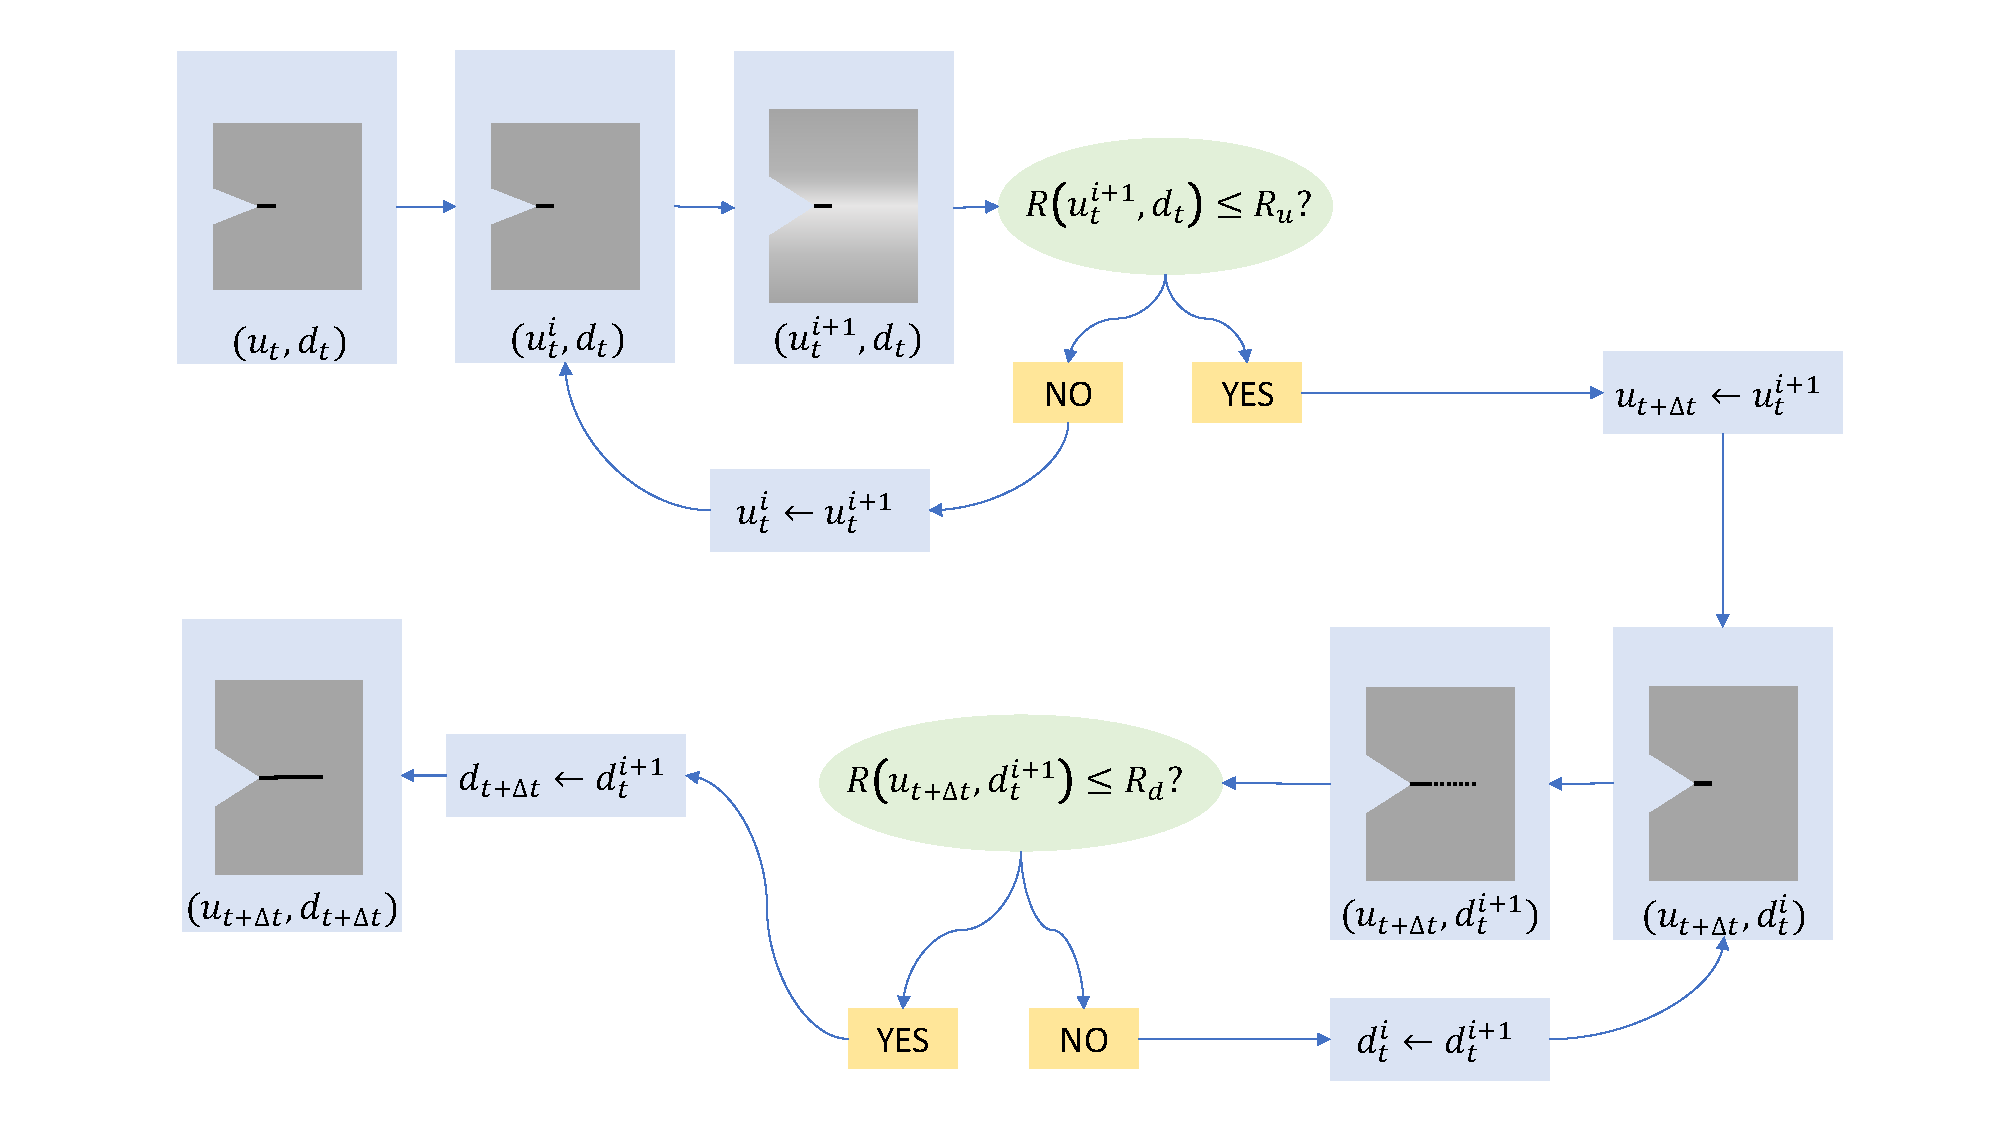
\includegraphics[width=7.cm]{img/time-staggered-resolution.pdf}
    \caption{Illustration of the time staggered resolution of Problem \ref{phase_field_lagrangian}}
    \label{time_staggered_resolution}
\end{figure}

% \begin{equation}
%     \left\{
%     \begin{aligned}
%     \ets{d}       &= \underset{d^{\star}\geq\bts{d}}{\argmin{}}\, \mathcal{L}\paren{\bts{\vec{u}},d^{\star}}\\
%     \ets{\vec{u}} &= \underset{\vec{u}^{\star}\in\text{C.A.}}{\argmin{}}\, \mathcal{L}\paren{\vec{u}^{\star},\ets{d}}
%     \end{aligned}
%     \right.
% \end{equation}

\begin{equation}
    \begin{cases}
        \begin{aligned}
            \tensoro{d}\vert_{t + \Delta t} = \min_{\hat{\tensoro{d}} \geq \tensoro{d}\vert_{t}}
            \mathcal{L}(\tensori{u}\vert_{t}, \hat{\tensoro{d}})
            \\
            \tensori{u}\vert_{t + \Delta t} = \min_{\hat{\tensori{u}} K.A.}
            \mathcal{L}(\hat{\tensori{u}}, \hat{\tensoro{d}}\vert_{t+ \Delta t})
        \end{aligned}
    \end{cases}
\end{equation}

\cite{miehe_phase_2010, nguyen_phase_2015, nguyen_phase-field_2016, molnar_2d_2017, molnar_open-source_2020}

\paragraph{\texttt{Cast3M} implementation}
\label{castem_implementation}

The idea that we followed is to integrate the damage update in the
mechanical iterations \cite{helfer_modelisation_2017}, \textit{i.e.} at each
iteration of the resolution of the mechanical resolution, update the
damage field as follows:

% \begin{equation}
%     \ets{d}^{(i+1)} = \underset{d^{\star}\geq\bts{d}}{\argmin{}}\, \mathcal{L}\paren{\ets{\vec{u}}^{(i)},d^{\star}}
% \end{equation}

\begin{equation}
    \tensoro{d}\vert_{t + \Delta t}^{i+1} = \min_{\hat{\tensoro{d}} \geq \tensoro{d}\vert_{t}}
    \mathcal{L}(\tensori{u}\vert_{t + \Delta t}^{i}, \hat{\tensoro{d}})
\end{equation}

where $i$ stands here for the iteration number of the mechanical
resolution.

Note that the convergence guarantees of the alternate minimisation
algorithm are lost.

\paragraph{Work of Ye Lu}

In his postdoctoral work, Ye Lu analyse the previous algorithm and
founds that the damage may become almost stationary during the
mechanical iterations \cite{lu_schema_2019}. However, he observed that even
small changes to the damage field perturbates the mechanical resolution,
slowing convergence and even leading to a stagnation of the mechanical
residual. He then proposed to freeze the damage field once it becomes
stationnary, a strategy that coined as "semi-implicit". Once the damage
field is freezed, the mechanical problem may be readily solved by a
standard Newton algorithm.

Note that the standard \texttt{Cast3M} algorithm, based on the initial elastic
stiffness, shows poor performances even when the damage field is
freezed.